\subsection{Data Preparation}
\label{sec:Data Preparation}

In the following section the data is prepared and cleaned up for training the model.

Data preparation is done in Python using multiple libraries. The same libraries
are also used in the modeling and evaluation stages of this project.
\emph{pandas} is used for storing and manipulating data in dataframes.
\emph{sklearn} is used for splitting data, creating validation curves,
transforming data and training the gradient boosting model.
\emph{matplotlib} and \emph{seaborn} are used for data visualization and plotting.
Additionaly \emph{numpy} is used for other operations on the data.

As with data collection, the complete code with documentation is attached in the appendix.

\subsubsection{Import and cleaning}


The CSV file is first imported and converted into a pandas dataframe.

\begin{lstlisting}[language=Python]
    df_import = pd.read_csv(os.path.join('..', 'data_collection', 'final_result.csv'))
\end{lstlisting}

Next, duplicates are removed. If there are two or more datapoints, which have the same value in their artist
and name column, only the first one is kept and all subsequent entries are removed.
This deduplication could also be done by using track ids. The drawback of this method is, that many artists
release their tracks multiple times, e.g. as a single and later in an album. These duplicates would not be
caught using the id, as different releases have different id values. As the artist and title doesn't change, almost
all duplicates are caught using artist and name.

\begin{lstlisting}[language=Python]
    df_dedup = df_import.drop_duplicates(subset=['categories.playlists.tracks.artists', 'categories.playlists.tracks.name'])
\end{lstlisting}

Next, all genres that are not to be used for training the model are filtered out.

\begin{lstlisting}[language=Python]
    genre_filter = ['hiphop', 'jazz', 'rock']
    df_filtered = df_dedup[df_dedup['categories.id'].isin(genre_filter)]
\end{lstlisting}

Then columns that are not needed for training are removed, including category name, all playlist information and
all track and album information. The category id is kept, as it will serve as the label.
The remaining columns are renamed, as the long JSON tree names are no longer needed.
The field \emph{category.id} is renamed to \emph{category} and each audio feature is renamed for example 
the danceability column is now called \emph{feature\_danceability}.
With unnecessary columns removed, a check is done to show any remaining null values.

\begin{lstlisting}[language=Python]
    df.isnull().sum()
\end{lstlisting}

In this dataset, there are no null values present.

The \emph{GradientBoostingClassifier} used for modeling only supports integer values as label input.
The category data is therefore encoded with integers using a custom function \emph{encode\_target}.
It takes a dataframe and the label column's name, than adds a "target" column with corresponding integer mappings.

\begin{lstlisting}[language=Python]
    def encode_target(df, target_column):

        df_mod = df.copy()
        map_to_int = {name: n for n, name in enumerate(df_mod["category"].unique())}
        df_mod["target"] = df_mod[target_column].replace(map_to_int)

        return (df_mod)

    df_target = encode_target(df, "category")
\end{lstlisting}

The head of the resulting dataframe is shown in table \ref{tbl:Dataframe after cleanup}.
The category to target integer mapping is shown in table \ref{tbl:Category to target integer mapping}.

\begin{table}[H]
    \centering
    \caption{Dataframe after cleanup}
    \label{tbl:Dataframe after cleanup}
%    \begin{tabular}{llrrrrrr}
%    \toprule
%    {} & category &  target &  feature\_danceability &  feature\_energy &  feature\_key &  feature\_loudness & ...\\ 
%    \midrule
%    0 &   hiphop &       0 &                 0.649 &           0.508 &            8 &           -10.232 & ...     \\ 
%    1 &   hiphop &       0 &                 0.849 &           0.631 &            3 &            -4.241 & ...     \\ 
%    2 &   hiphop &       0 &                 0.793 &           0.481 &            9 &            -9.258 & ...     \\ 
%    3 &   hiphop &       0 &                 0.875 &           0.478 &            7 &           -10.562 & ...     \\ 
%    4 &   hiphop &       0 &                 0.684 &           0.624 &            2 &            -7.414 & ...     \\ 
%    5 &   hiphop &       0 &                 0.762 &           0.649 &           11 &            -5.624 & ...     \\ 
%    \bottomrule
%    \toprule
%    ... & feature\_mode &  feature\_speechiness &  feature\_acousticness &  feature\_instrumentalness &  feature\_liveness &  feature\_valence &  feature\_tempo \\
%    \midrule
%    1 &               0.0959 &               0.03450 &                  0.000036 &            0.0736 &            0.405 &        157.975 &         
%    0 &               0.0637 &               0.17100 &                  0.000000 &            0.1490 &            0.550 &        135.997 &         
%    1 &               0.1240 &               0.01900 &                  0.000001 &            0.1390 &            0.395 &        132.202 &         
%    1 &               0.2180 &               0.00717 &                  0.000000 &            0.1470 &            0.409 &        128.990 &         
%    0 &               0.3470 &               0.23900 &                  0.000000 &            0.1120 &            0.708 &        146.925 &         
%    0 &               0.0527 &               0.58000 &                  0.000017 &            0.0971 &            0.501 &        145.090 &         
%\bottomrule
%
%      194051 &                       4 \\
%      215304 &                       4 \\
%      204626 &                       4 \\
%      200959 &                       4 \\bular}
%      156735 &                       4 \\
%      239146 &                       4 \\

%    \end{tabular}
\end{table}
\textbf{Hier Category/target mapping table}

\label{tbl:Category to target integer mapping}

Looking at the number of samples per category (tabel \ref{tbl:Samples per category} reveals, that the dataset
is very uneven, with more than half of the samples being in the category \emph{rock}.

\textbf{Hier samples per category}

As explained in section \ref{sec:Mean Removal, Variance Scaling and Standardization} and \ref{sec:Dimension Reduction}
methods like standardization and \ac{PCA} can have a positive impact on the models accuracy.
Before finding the best model using hyperparameter tuning, the best form of input data is evaluated by transforming
the data in different ways and training a Gradient Boosting model using the default parameters specified in sklearn.
This way, the best form of input data can be found without the overhead of resource intensive grid search.

To be able to easily train models using different forms of input data, a method \emph{eval\_prep} was created,
which takes a dataframe, a list of all feature column names and the label column name. It then splits the dataframe
into train and test sets, trains a \emph{GradientBoostingClassifier} and returns a simple accuracy score.
This process is explained in depth in the modeling section.

First, the regular dataframe is used as input data, resulting in an accuracy score of $0.8505$.

\begin{lstlisting}[language=Python]
    score = eval_prep(df, features, "target")
\end{lstlisting}

\subsubsection{Data Transformation}

Next, mean removal, variance scaling and standardisation are attempted, by using the \emph{StandardScaler}
class from sklearn to transform the data. The code for standardization is shown below.
Mean removal and variance scaling use the same class with additional parameters.

\begin{lstlisting}[language=Python]
    X_s = df[features]
    y = df["target"]

    X_s = StandardScaler().fit_transform(X_s)

    df_s = pd.DataFrame(data=X_s)
    df_s.insert(0, "target", y)
    df_s.columns = ["target"] + features

    score = eval_prep(df_s, features, "target")
\end{lstlisting}

This results in the following scores, beating the untransformed data in all cases.

\begin{itemize}
    \item Mean Removal: $0.8509$
    \item Variance Scaling: $0.8520$
    \item Standardization: $0.8523$
\end{itemize}

\subsubsection{Principal Component Analysis}

Next \ac{PCA} is attempted using sklearns \emph{PCA} class. It is able to take any dataset and reduce
its dimensionality to any number of dimensions. The dimensionality is reduced to all dimensions
between 2 and 13 to see, which dimensionality results in the best score.
\ac{PCA} was done both on the raw dataset and in combination with standardized data (both before and afterwards).

\ac{PCA} does not yield good results with this dataset. The score for all of the combination is always worse
than using untransformed data. 
The PCA score was best when keeping 13 dimensions, declining further when removing more dimensions.
These are the scores using each combination with PCA and keeping 13 dimensions:

\begin{itemize}
    \item PCA only with 13 components: $0.8352$
    \item Standardization after PCA with 13 components: $0.8348$
    \item Standardization before PCA with 13 components: $0.8277$
\end{itemize}

Figure \ref{fig:Score for each PCA dimensionality} shows the test accuracy using PCA on the untransformed data
for each number of components.

\begin{figure}[H]
    \caption{Test accuracy for each dimensionality after PCA}
	\label{fig:Score for each PCA dimensionality}
    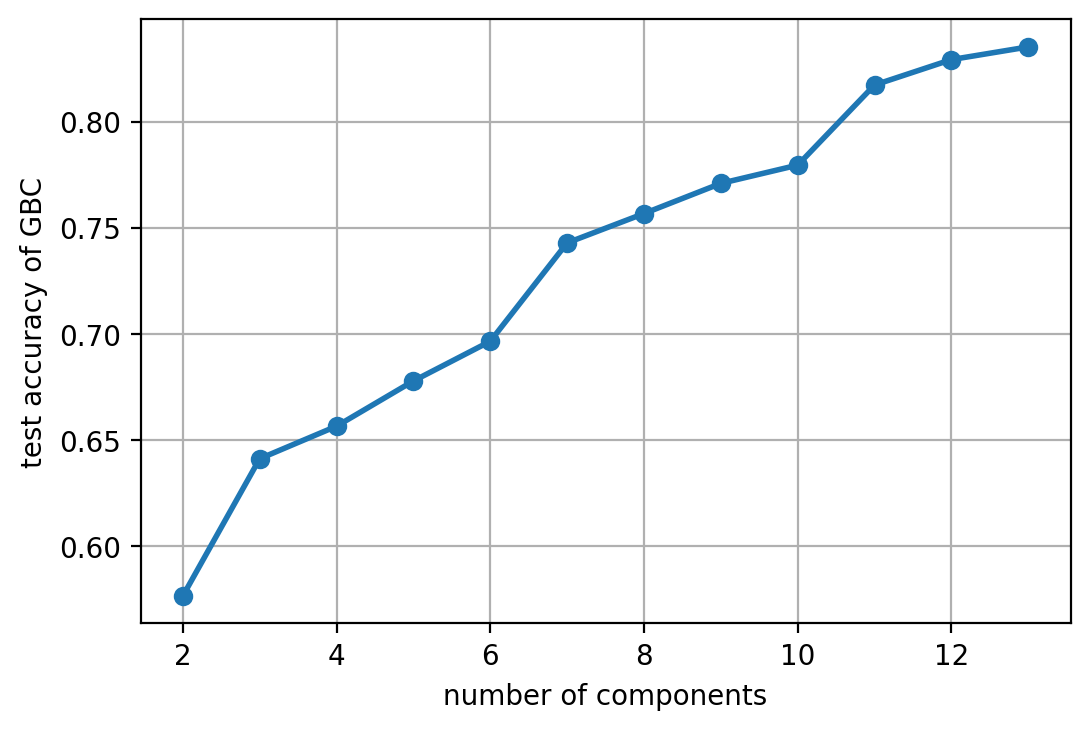
\includegraphics[width=0.6\textwidth]{dimensionality_PCA}
\end{figure}

As the results using \ac{PCA} do not improve the score, the code is not shown here.
Testing data transformation and dimension reduction with this dataset and a default \emph{GradientBoostingClassifier}
shows, that the model benefits slightly from standardized data, improving the overall score compared to the raw dataset
by $0.19\%$. Therefore, standardized data is used going forward.


%Now that all columns needed for training the model are prepared, the dataset needs to be split in 
%test and training data. This is necessary to be able to calculate an accuracy score for the model after training.
%In order to calculate this score, data is needed that the model has never seen before, which ensures that 
%the score is not just a result of overfitting, but the accuracy would be the same on real world data.
%For splitting the data, the function \emph{train\_test\_split} from sklearn is used.
%First the dataset is shuffled so each set contains a near equal amount of entries for each genre.
%Then the shuffled dataset is split, with an 80\% of samples going into the training set and 20\% going 
%into the test set. This results in 10.701 rows of training data and 2.676 rows of test data.
%
%\begin{lstlisting}[language=Python]
%    from sklearn.model_selection import train_test_split
%    df_target_shuffled = df_target.sample(frac=1, random_state=45)
%    train, test = train_test_split(df_target_shuffled, test_size=0.2, random_state=45, shuffle=False)
%\end{lstlisting}
%
%Next, features and labels are split into seperate datasets. This is necessary, because the GradientBoostingClassifiers
%fit method takes features and labels as seperate arguments called X for input and y for label. Datapoints are matched by their row numbers.
%Labels are stored in a list containing all values from the target column like so.
%
%\begin{lstlisting}[language=Python]
%    # y contains list of target values
%    y_train = train["target"]
%    y_test = test["target"]
%    y_all = df_target_shuffled["target"]
%\end{lstlisting}
%
%The features are stored in dataframes. The columns are selected using a list of all column names which contain features
%and then creating a new dataset only containing those columns:
%
%\begin{lstlisting}[language=Python]
%    # columns 1 to 14 contain the features, column 0 is the category and 15 the target
%    features = list(train.columns[1:14])
%
%    # create datasets only containing feature columns
%    X_train = train[features]
%    X_test = test[features]
%    X_all = df_target_shuffled[features]
%\end{lstlisting}
%
%At this point, all data has been cleaned up, targets have been generated, it has been split into training and test data and
%features have been seperated from labels. The data is now ready for training the model.